\chapter{Implementation}
This chapter will go through implementing the Ezuino programming language. The programming language is done, and we can group the different implementation topics. First, we will go through the build Abstract Syntax Tree (AST) visitor class and then move to type checker, where we provide each node in the AST a type. Then we will go through the different visitors and code generation visitors. Finally, we will go through the error handler, which provides an error overview for the users.
\section{Type checker}
The type checker implements the semantic rules of Ezuino specified in chapter \ref{semantics}. \\
We split the type checker into two visitors TypeCheckerVisitor and ReturnStatementVisitor. TypeCheckerVisitor checks that the condition in a boolean statement has the correct type and that expressions are legal. ReturnStatementVisitor ensures that the actual returned value of a program matches the type defined in the function declaration.
The way TypeCheckerVisitor type checks expressions is through a setup where every expression node extends that inherits from an interface called ITypeNode. The ITypeNode interface requires that every child class have the method for getting and setting a type attribute. When type checking happens, we then compare each node through the checkType method.
\begin{figure}[H]
\centering
\frame{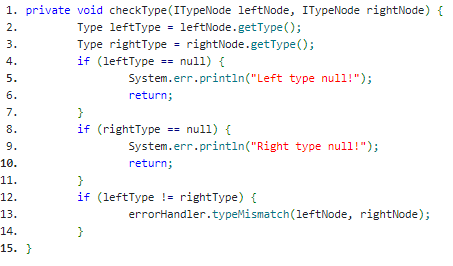
\includegraphics[scale=1.0]{figures/implementation/typeCecker/5-check-type.png}}
\caption{}
\label{dadsa}
\end{figure}

The boolean condition is checked in an if- and else statements.
 \begin{figure}[H]
\centering
\frame{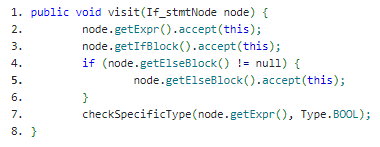
\includegraphics[scale=1.0]{figures/implementation/typeCecker/2-if-stmt.png}}
\caption{}
\label{lf05}
\end{figure}

An example of typechecking expressions. When an additive expression is reached both nodes are type checked.
\begin{figure}[H]
\centering
\frame{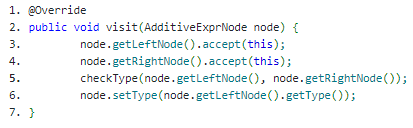
\includegraphics[scale=1.0]{figures/implementation/typeCecker/4-additive-typecheck.png}}
\caption{}
\label{lf05}
\end{figure}

In a unaryexpression it is also necessary to check that the operations performed are done with legal types. This is done through an switch case so it is easy to extend if more unary expressions needs to be added in the future. 
\begin{figure}[H]
\centering
\frame{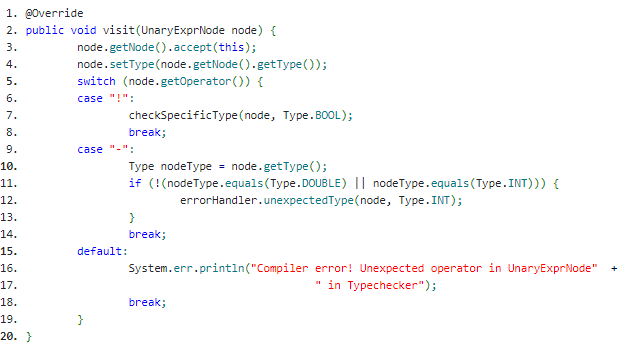
\includegraphics[scale=1.0]{figures/implementation/typeCecker/6-unary-expr.png}}
\caption{}
\label{lf05}
\end{figure}

When a return statement is returned it is set to its expression, this is important for type checking the return statement with the function declaration later in ReturnStatementVisitor.
It is also here that return in void functions is implemented. If a return statement has no value,we assume it to be a void function. This in practice makes the return key-word a way to preemptively end void functions.
\begin{figure}[H]
\centering
\frame{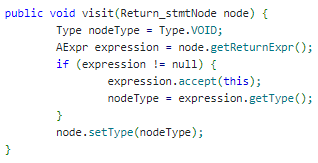
\includegraphics[scale=1.0]{figures/implementation/typeCecker/1-return-type.png}}
\caption{}
\label{lf05}
\end{figure}
This is the ReturnSatementVisitor. When a function is declared the type, it was declared as is temporarily saved in a symbol table. When a return statement is reached, the return statements type is compared with a type of the last function that was declared which was saved in the symbol table within that scope. This ensures that if there are several nested function declarations, the return type is compared to the most recent “active” scope.
\begin{figure}[H]
\centering
\frame{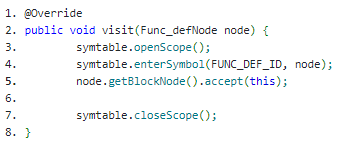
\includegraphics[scale=1.0]{figures/implementation/typeCecker/2-1-func-def.png}}
\caption{}
\label{lf05}
\end{figure}
 \begin{figure}[H]
\centering
\frame{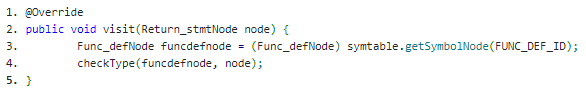
\includegraphics[scale=1.0]{figures/implementation/typeCecker/2-2-return-type-check.png}}
\caption{}
\label{lf05}
\end{figure}


\section{Checking that return are guaranteed}
If an function is not a void function, it should only be legal if it is guaranteed that it will reach an return statement. This means that if there is no return statement in the scope of the definition body, it must be because there is an if- and else block in the scope of the body where every if statement and the else statement have an return statement. 

\begin{figure}[H]
\centering
\frame{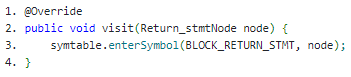
\includegraphics[scale=1.0]{figures/implementation/typeCecker/3-3-return-stmt-enter-symbol-table.png}}
\caption{If a return statement is encountered it, it is noted for the current scope.}
\label{lf05}
\end{figure}

\begin{figure}[H]
\centering
\frame{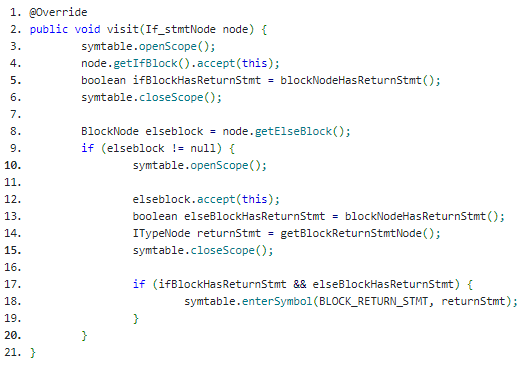
\includegraphics[scale=1.0]{figures/implementation/typeCecker/3-2-ifstmt-return-check.png}}
\caption{If an return statement in an if else block is guaranteed, it is noted for the current scope.} 
\label{lf05}
\end{figure}

 \begin{figure}[H]
\centering
\frame{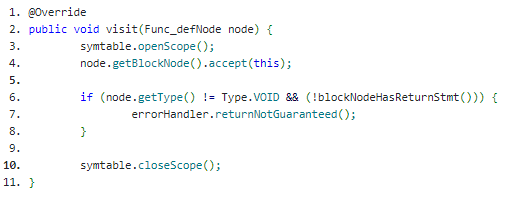
\includegraphics[scale=1.0]{figures/implementation/typeCecker/3-1-func-def-missing-return.png}}
\caption{If there is no return statement in the current scope, or an if else block where return is guaranteed throw an error.}
\label{lf05}
\end{figure}


\section{Function Structure Visitor}
The purpose of this section is to explain, how the Ezuino compiler guarantee that any function called, always has the correct structure for the given function (note: before a function can be called, it must have been declared first. Except for predefined functions such as Arduino functions).
\\\\
To accomplish this goal the Ezuino compiler implements a Visitor named: "FuncStructureVisitor". The goal for this Visitor is to verify that all functions called in a given program, always has the same structure as the function declaration. This is also true for the predefined Arduino functions. However, since these are predefined by the compiler, the structure of these functions are hard coded into the Visitor.
\\\\
Exactly like the other Visitors in the compiler the FuncStructureVisitor runs through the generated AST, starting at the first node and visiting all of it's children nodes.\\
The nodes that mainly will be affected by the FuncStructureVisitor, is the nodes that has to do with functions. Specifically these nodes are function declarations, function calls and predefined functions such as Arduino functions.
\\\\
Listing \ref{FuncDefNode} shows how a function declaration node is handled by the visitor. Since the node is a function declaration, the node must be store in a symbol table for the current scope. this is done so that when the visitor meets the function call node, it can look up in the symbol table to find how the function was declared.\\
As seen on line 3, the function declaration is stored in the symbol table with the function id and the node.
\begin{lstlisting}[caption={Visit method for FuncDefNode in FuncStructureVisitor}, label={FuncDefNode}]
    $$@Override
    public void visit(Func_defNode node) {
        symtable.enterSymbol(node.getId(), node);
        node.getBlockNode().accept(this);
    }
\end{lstlisting}
\noindent\newline
Listing \ref{customFuncCall} shows how a custom function call is handled by the visitor. The name CustomFuncCall tells us that this is not one of the predefined functions in the compiler, but instead a function that has been declared by a user.\\
Since this is a custom function call, the compiler does not know what the structure of the function is. therefore it must search the symbol table for a function with the same id as the call.\\
Once the correct declaration has been found, the visitor compares the parameters of the function call with the parameters of the function declaration. If these does not match, an error is thrown to the errorHandler.\\
Similarly if the visitor cannot find a function declaration with the same id as the function call, an error is thrown to the errorHandler.
\begin{lstlisting}[caption={Visit method for CustomFuncCallStmtNode in FuncStructureVisitor}, label={customFuncCall}]
$$@Override
public void visit(CustomFuncCallStmtNode node) {
    Func_defNode funcdef = (Func_defNode) symtable.retrieveSymbol(node.getId());
    matchParameterList(node.getId(), node.getParameters(), funcdef.getParameters());
\end{lstlisting}
\noindent\newline
Listing \ref{matchParameterList} is the private helper method, which compares parameters of function calls. It is the same method used in line 4 of listing \ref{customFuncCall}.\\
As the function structure visitor's job is to verify that the structure of function is correct, this private method is one of the core functions of the visitor.\\
The idea behind verifying the structure of functions, is to compare the types of the parameters of the function. This involves comparing the parameters of the function call and the function declaration. For the function call to be correct, the parameters must match the parameters of the function declaration.\\
To do this, the method takes a list of function call parameters and a list of function declaration parameters as input.
\\\\
Firstly the method compares the number of parameters of both the call and declaration. If they are not the same, an error has occurred and is thrown to the errorHandler. This happens on line 3-5 of the listing.\\
Secondly it compares the types of the parameters, in order, of both the call and declaration. If they are not the same, an error has occurred and is thrown to the errorHandler. This happens on line 7-11 of the listing.
\begin{lstlisting}[caption={Private helper method for verifying function parameters in FuncStructureVisitor}, label={matchParameterList}]
    private void matchParameterList(String functionname, List<AExpr> callparams, List<DclNode> defparams) {
        int parametercount = callparams.size();
        if (parametercount != defparams.size()) {
            errorHandler.parameterLengthError(functionname);
            return;
        }
        for (int i = 0; i < parametercount; i++) {
            AExpr callParam = callparams.get(i);
            DclNode dclnode = defparams.get(i);
            if (callParam.getType() != dclnode.getType()) {
                errorHandler. parameterTypeError(functionname);
            }
        }
    }
\end{lstlisting}
\noindent\newline
Listing \ref{AnalogReadNode} is an example of a predefined function in the compiler and shows how the visitor generally handles predefined function calls.\\
In this case the function call is to AnalogRead, which is an Arduino specified function. In the case of AnalogRead, it is necessary to perform an additional check for the size of the int parameter. The additional check occurs on line 8. This check is not present for all predefined functions, but for AnalogRead it is needed to compatible with Arduino's 8 bit int size.
\\\\
The idea behind verifying predefined function calls is that, because the function is predefined, the compiler already knows what parameters are required for the call. Predefined functions Therefore have hard coded parameters, which cannot be changed on compile time.\\
As seen on line 3, the expected type of the AnalogRead function is an int, and since there is only one type, the function only takes one parameter.\\
Additionally the parameter must be held within either an IntegerLiteral node or IdNode. This is to ensure that only the correct int node is the parameter for the function call. This occurs on line 5-6.\\
Lastly a call to compare the parameters is made on line 9.
\begin{lstlisting}[caption={Visit method for AnalogReadNode in FuncStructureVisitor}, label={AnalogReadNode}]
$$@Override
public void visit(AnalogReadNode node) {
    Type[] expectedType = {Type.INT};
    AExpr firstParam = node.getParameters().get(0);
    if (!(firstParam instanceof IntegerLiteral || firstParam instanceof IdNode)) {
        errorHandler. invalidFunctionParameterError(node.getID());
    }
    checkArduinoRange(firstParam);
    checkFuncParameters(node.getID(), node.getParameters(), 1, expectedType);
}
\end{lstlisting}
\noindent\newline
Listing \ref{checkFuncParameters} shows the private helper method for comparing predefined function parameters. Similarly to the private method in listing \ref{matchParameterList}, the purpose of the checkFuncParameters method is to verify function calls and therefore also a core part of the visitor.\\
The idea for the checkFuncParameters method is the same as the matchParameterList. It compares a list of parameters with a list of types, and for the function call to be correct, the parameters must match the predefined parameters.
\\\\
Firstly the method confirms that the amount of parameters is the same as required. If they are not the same, the function call is incorrect and an error is thrown to the errorHandler. This occurs on line 2-3.\\
Secondly the method verifies that the parameters have the correct types in the correct order.\\
This is done by calling another helper method, which just compares two types. If the two types are not the same, an error is thrown to the errorHandler. This occurs on line 5-7.
\begin{lstlisting}[caption={Private helper method for verifying predefined function parameters in FuncStructureVisitor}, label={checkFuncParameters}]
private void checkFuncParameters(String nodeId, List<AExpr> parameters, int requiredParameters, Type[] typeList) {
    if (parameters.size() != requiredParameters) {
        errorHandler.parameterLengthError(nodeId);
    }
    for (int i = 0; i < requiredParameters; i++) {
        if (parameters.get(i) != null) {
            checkSpecificType(parameters.get(i), typeList[i]);
        }
    }
}
\end{lstlisting}
\noindent\newline
The five listings of code looked at in this section, should give a good idea about how the Function Structure Visitor works.\\
As a basic idea, the Visitor works by visiting nodes in the AST and depending on which node it visits, verifies if the function function structure matches the declared or defined structure.
\\\\
There are three types of nodes which specifically has to do with functions. Depending on the node, a different check is preformed to verify the function structure.
\begin{enumerate}
    \item Function declarations, where nodes are stored for later comparisons.
    \item Custom function calls and function expression calls, both of which falls under the same type. These are used for users to call their own declared functions.
    \item Predefined functions, such as Print, AnalogRead and other Arduino functions.
\end{enumerate}
For custom function calls, their parameters are compared to their declaration. Predefined functions are compared to the compiler's required types.\\
If no errors occur, it means that every function in the program is used correctly.